\documentclass[12pt,superscriptaddress]{revtex4-2}
\usepackage[dvips]{graphicx}
\usepackage{amsmath,amssymb,bm}
\usepackage{color}
\usepackage{mathrsfs}
\usepackage{setspace}

%\usepackage{amsmath,amsthm,amscd,amssymb}
\usepackage[colorlinks=true
,breaklinks=true
,urlcolor=blue
,anchorcolor=blue
,citecolor=blue
,filecolor=blue
,linkcolor=blue
,menucolor=blue
,linktocpage=true]{hyperref}
\hypersetup{
bookmarksopen=true,
bookmarksnumbered=true,
bookmarksopenlevel=10
}
\usepackage[noBBpl,sc]{mathpazo}
\usepackage[papersize={7.0in, 10.0in}, left=.5in, right=.5in, top=1in, bottom=.9in]{geometry}
\linespread{1.05}
\sloppy
\raggedbottom
\pagestyle{plain}

% these include amsmath and that can cause trouble in older docs.
\makeatletter
\@ifpackageloaded{amsmath}{}{\RequirePackage{amsmath}}

\DeclareFontFamily{U}  {cmex}{}
\DeclareSymbolFont{Csymbols}       {U}  {cmex}{m}{n}
\DeclareFontShape{U}{cmex}{m}{n}{
    <-6>  cmex5
   <6-7>  cmex6
   <7-8>  cmex6
   <8-9>  cmex7
   <9-10> cmex8
  <10-12> cmex9
  <12->   cmex10}{}

\def\Set@Mn@Sym#1{\@tempcnta #1\relax}
\def\Next@Mn@Sym{\advance\@tempcnta 1\relax}
\def\Prev@Mn@Sym{\advance\@tempcnta-1\relax}
\def\@Decl@Mn@Sym#1#2#3#4{\DeclareMathSymbol{#2}{#3}{#4}{#1}}
\def\Decl@Mn@Sym#1#2#3{%
  \if\relax\noexpand#1%
    \let#1\undefined
  \fi
  \expandafter\@Decl@Mn@Sym\expandafter{\the\@tempcnta}{#1}{#3}{#2}%
  \Next@Mn@Sym}
\def\Decl@Mn@Alias#1#2#3{\Prev@Mn@Sym\Decl@Mn@Sym{#1}{#2}{#3}}
\let\Decl@Mn@Char\Decl@Mn@Sym
\def\Decl@Mn@Op#1#2#3{\def#1{\DOTSB#3\slimits@}}
\def\Decl@Mn@Int#1#2#3{\def#1{\DOTSI#3\ilimits@}}

\let\sum\undefined
\DeclareMathSymbol{\tsum}{\mathop}{Csymbols}{"50}
\DeclareMathSymbol{\dsum}{\mathop}{Csymbols}{"51}

\Decl@Mn@Op\sum\dsum\tsum

\makeatother

\makeatletter
\@ifpackageloaded{amsmath}{}{\RequirePackage{amsmath}}

\DeclareFontFamily{OMX}{MnSymbolE}{}
\DeclareSymbolFont{largesymbolsX}{OMX}{MnSymbolE}{m}{n}
\DeclareFontShape{OMX}{MnSymbolE}{m}{n}{
    <-6>  MnSymbolE5
   <6-7>  MnSymbolE6
   <7-8>  MnSymbolE7
   <8-9>  MnSymbolE8
   <9-10> MnSymbolE9
  <10-12> MnSymbolE10
  <12->   MnSymbolE12}{}

\DeclareMathSymbol{\downbrace}    {\mathord}{largesymbolsX}{'251}
\DeclareMathSymbol{\downbraceg}   {\mathord}{largesymbolsX}{'252}
\DeclareMathSymbol{\downbracegg}  {\mathord}{largesymbolsX}{'253}
\DeclareMathSymbol{\downbraceggg} {\mathord}{largesymbolsX}{'254}
\DeclareMathSymbol{\downbracegggg}{\mathord}{largesymbolsX}{'255}
\DeclareMathSymbol{\upbrace}      {\mathord}{largesymbolsX}{'256}
\DeclareMathSymbol{\upbraceg}     {\mathord}{largesymbolsX}{'257}
\DeclareMathSymbol{\upbracegg}    {\mathord}{largesymbolsX}{'260}
\DeclareMathSymbol{\upbraceggg}   {\mathord}{largesymbolsX}{'261}
\DeclareMathSymbol{\upbracegggg}  {\mathord}{largesymbolsX}{'262}
\DeclareMathSymbol{\braceld}      {\mathord}{largesymbolsX}{'263}
\DeclareMathSymbol{\bracelu}      {\mathord}{largesymbolsX}{'264}
\DeclareMathSymbol{\bracerd}      {\mathord}{largesymbolsX}{'265}
\DeclareMathSymbol{\braceru}      {\mathord}{largesymbolsX}{'266}
\DeclareMathSymbol{\bracemd}      {\mathord}{largesymbolsX}{'267}
\DeclareMathSymbol{\bracemu}      {\mathord}{largesymbolsX}{'270}
\DeclareMathSymbol{\bracemid}     {\mathord}{largesymbolsX}{'271}

\def\horiz@expandable#1#2#3#4#5#6#7#8{%
  \@mathmeasure\z@#7{#8}%
  \@tempdima=\wd\z@
  \@mathmeasure\z@#7{#1}%
  \ifdim\noexpand\wd\z@>\@tempdima
    $\m@th#7#1$%
  \else
    \@mathmeasure\z@#7{#2}%
    \ifdim\noexpand\wd\z@>\@tempdima
      $\m@th#7#2$%
    \else
      \@mathmeasure\z@#7{#3}%
      \ifdim\noexpand\wd\z@>\@tempdima
        $\m@th#7#3$%
      \else
        \@mathmeasure\z@#7{#4}%
        \ifdim\noexpand\wd\z@>\@tempdima
          $\m@th#7#4$%
        \else
          \@mathmeasure\z@#7{#5}%
          \ifdim\noexpand\wd\z@>\@tempdima
            $\m@th#7#5$%
          \else
           #6#7%
          \fi
        \fi
      \fi
    \fi
  \fi}

\def\overbrace@expandable#1#2#3{\vbox{\m@th\ialign{##\crcr
  #1#2{#3}\crcr\noalign{\kern2\p@\nointerlineskip}%
  $\m@th\hfil#2#3\hfil$\crcr}}}
\def\underbrace@expandable#1#2#3{\vtop{\m@th\ialign{##\crcr
  $\m@th\hfil#2#3\hfil$\crcr
  \noalign{\kern2\p@\nointerlineskip}%
  #1#2{#3}\crcr}}}

\def\overbrace@#1#2#3{\vbox{\m@th\ialign{##\crcr
  #1#2\crcr\noalign{\kern2\p@\nointerlineskip}%
  $\m@th\hfil#2#3\hfil$\crcr}}}
\def\underbrace@#1#2#3{\vtop{\m@th\ialign{##\crcr
  $\m@th\hfil#2#3\hfil$\crcr
  \noalign{\kern2\p@\nointerlineskip}%
  #1#2\crcr}}}

\def\bracefill@#1#2#3#4#5{$\m@th#5#1\leaders\hbox{$#4$}\hfill#2\leaders\hbox{$#4$}\hfill#3$}

\def\downbracefill@{\bracefill@\braceld\bracemd\bracerd\bracemid}
\def\upbracefill@{\bracefill@\bracelu\bracemu\braceru\bracemid}

\DeclareRobustCommand{\downbracefill}{\downbracefill@\textstyle}
\DeclareRobustCommand{\upbracefill}{\upbracefill@\textstyle}

\def\upbrace@expandable{%
  \horiz@expandable
    \upbrace
    \upbraceg
    \upbracegg
    \upbraceggg
    \upbracegggg
    \upbracefill@}
\def\downbrace@expandable{%
  \horiz@expandable
    \downbrace
    \downbraceg
    \downbracegg
    \downbraceggg
    \downbracegggg
    \downbracefill@}

\DeclareRobustCommand{\overbrace}[1]{\mathop{\mathpalette{\overbrace@expandable\downbrace@expandable}{#1}}\limits}
\DeclareRobustCommand{\underbrace}[1]{\mathop{\mathpalette{\underbrace@expandable\upbrace@expandable}{#1}}\limits}

\makeatother


% make sure there is enough TOC for reasonable pdf bookmarks.
\setcounter{tocdepth}{3}

%\usepackage[dotinlabels]{titletoc}
%\titlelabel{{\thetitle}.\quad}
%\usepackage{titletoc}
\usepackage[small]{titlesec}

\titleformat{\section}[block]
  {\fillast\medskip}
  {\bfseries{\thesection. }}
  {1ex minus .1ex}
  {\bfseries}
 
\titleformat*{\subsection}{\itshape}
\titleformat*{\subsubsection}{\itshape}

\setcounter{tocdepth}{2}

\titlecontents{section}
              [2.3em] 
              {\bigskip}
              {{\contentslabel{2.3em}}}
              {\hspace*{-2.3em}}
              {\titlerule*[1pc]{}\contentspage}
              
\titlecontents{subsection}
              [4.7em] 
              {}
              {{\contentslabel{2.3em}}}
              {\hspace*{-2.3em}}
              {\titlerule*[.5pc]{}\contentspage}

% hopefully not used.           
\titlecontents{subsubsection}
              [7.9em]
              {}
              {{\contentslabel{3.3em}}}
              {\hspace*{-3.3em}}
              {\titlerule*[.5pc]{}\contentspage}
%\makeatletter
\renewcommand\tableofcontents{%
    \section*{\contentsname
        \@mkboth{%
           \MakeLowercase\contentsname}{\MakeLowercase\contentsname}}%
    \@starttoc{toc}%
    }
\def\@oddhead{{\scshape\rightmark}\hfil{\small\scshape\thepage}}%
\def\sectionmark#1{%
      \markright{\MakeLowercase{%
        \ifnum \c@secnumdepth >\m@ne
          \thesection\quad
        \fi
        #1}}}
        
\makeatother

%\makeatletter

 \def\small{%
  \@setfontsize\small\@xipt{13pt}%
  \abovedisplayskip 8\p@ \@plus3\p@ \@minus6\p@
  \belowdisplayskip \abovedisplayskip
  \abovedisplayshortskip \z@ \@plus3\p@
  \belowdisplayshortskip 6.5\p@ \@plus3.5\p@ \@minus3\p@
  \def\@listi{%
    \leftmargin\leftmargini
    \topsep 9\p@ \@plus3\p@ \@minus5\p@
    \parsep 4.5\p@ \@plus2\p@ \@minus\p@
    \itemsep \parsep
  }%
}%
 \def\footnotesize{%
  \@setfontsize\footnotesize\@xpt{12pt}%
  \abovedisplayskip 10\p@ \@plus2\p@ \@minus5\p@
  \belowdisplayskip \abovedisplayskip
  \abovedisplayshortskip \z@ \@plus3\p@
  \belowdisplayshortskip 6\p@ \@plus3\p@ \@minus3\p@
  \def\@listi{%
    \leftmargin\leftmargini
    \topsep 6\p@ \@plus2\p@ \@minus2\p@
    \parsep 3\p@ \@plus2\p@ \@minus\p@
    \itemsep \parsep
  }%
}%
\def\open@column@one#1{%
 \ltxgrid@info@sw{\class@info{\string\open@column@one\string#1}}{}%
 \unvbox\pagesofar
 \@ifvoid{\footsofar}{}{%
  \insert\footins\bgroup\unvbox\footsofar\egroup
  \penalty\z@
 }%
 \gdef\thepagegrid{one}%
 \global\pagegrid@col#1%
 \global\pagegrid@cur\@ne
 \global\count\footins\@m
 \set@column@hsize\pagegrid@col
 \set@colht
}%

\def\frontmatter@abstractheading{%
\bigskip
 \begingroup
  \centering\large
  \abstractname
  \par\bigskip
 \endgroup
}%

\makeatother

%\DeclareSymbolFont{CMlargesymbols}{OMX}{cmex}{m}{n}
%\DeclareMathSymbol{\sum}{\mathop}{CMlargesymbols}{"50}
\def\beq{\begin{equation}}
\def\eeq{\end{equation}}
\def\beqn{\begin{eqnarray}}
\def\eeqn{\end{eqnarray}}
\def\slash{/\hspace*{-2.2mm}}
\newcommand{\intsum}{
\hspace*{1mm}{\mbox{\Large$\Sigma$}}\hspace*{-4.2mm}\int}
\makeatletter
\newcommand\be{\@ifstar{\[}{\begin{equation}}}
\newcommand\ee{\@ifstar{\]}{\end{equation}}}
\makeatother
\newcommand\bp{\begin{pmatrix}}
\newcommand\ep{\end{pmatrix}}
\newcommand\ua{\uparrow}
\newcommand\da{\downarrow}
\newcommand{\ket}[1]{\left| #1 \right\rangle}
\newcommand{\bra}[1]{\left\langle #1 \right|}
\newtheorem{theorem}{Theorem}

\begin{document}
\title{Supermeasured: Violating Statistical Independence without violating statistical independence}
\author{T.N.\ Palmer}
\affiliation{Department of Physics, University of Oxford, UK}
\email{tim.palmer@physics.ox.ac.uk}
\author{S.\ Hossenfelder}
\affiliation{Frankfurt Institute for Advanced Studies, Ruth-Moufang-Str. 1, D-60438 Frankfurt am Main, Germany}
\author{J.R.\ Hance}
\affiliation{Quantum Engineering Technology Laboratories, Department of Electrical and Electronic Engineering, University of Bristol, Woodland Road, Bristol, BS8 1US, UK}
\date{\today}

\begin{abstract}
Bell's theorem is often said to imply that quantum mechanics violates local causality, and that local causality cannot be restored with a hidden-variables theory. This however is only correct if the hidden-variables theory fulfils an assumption called Statistical Independence. Violations of Statistical Independence are commonly interpreted as correlations between the measurement settings and the hidden variables (which determine the measurement outcomes). Such correlations have been discarded as ``finetuning'' or a ``conspiracy''. We here point out that the common interpretation is at best physically ambiguous and at worst incorrect. The problem with the common interpretation is that Statistical Independence might be violated because of a non-trivial measure in state space, a possibility we propose to call ``supermeasured''. We use Invariant Set Theory as an example of a supermeasured theory that violates the Statistical Independence assumption in Bell's theorem without requiring correlations between hidden variables and measurement settings. 
\end{abstract}

\maketitle

\newpage

\section{Introduction}
\label{intro}
Bell's theorem \cite{Bell1964OnEPR} has been a milestone in our understanding of quantum mechanics by detailing just what correlations are necessary to reproduce observations. Unfortunately, many physicists have jumped to incorrect conclusions from it. A 2016 survey among professional physicists \cite{Sujeevan2016Survey} found that 34\% believe Bell's theorem shows that ``Hidden variables are impossible,'' that is, they think Bell's theorem rules out theories in which measurement outcomes are determined by variables that are not accounted for in standard quantum mechanics. Similarly, in a survey conducted among professional quantum physicists at a conference in 2012 \cite{Schlosshauer2013Attitudes}, 64\% claimed that Bell's theorem rules out hidden variable theories (and said local realism is untenable). This is of course not so. Bell's theorem merely shows that a hidden variables theory {\emph{which fulfills all the assumptions of the theorem}} is ruled out by observation.

Bell's theorem however contains one questionable assumption: Statistical Independence, sometimes called the ``Free Will'' or ``Free Choice'' assumption (here capitalised to distinguish it from the intuitive ideas of statistical independence, free will and free  choice).
Indeed, one can interpret \emph{all} experiments that have found violations of Bell's inequality as simply demonstrating that if quantum mechanics is underpinned by a local, causal, and deterministic theory, then that underlying theory must violate Statistical Independence. Clearly the conclusion to draw from this is that we should look for a hidden-variables theory that violates Statistical Independence, not least to develop a quantum formalism that is compatible with General Relativity. 
Of course this is not historically what has happened. Instead, physicists have collectively discarded the possibility that Statistical Independence might be violated because they misunderstood what it means. For example, referring to Statistical Independence as ``free will'' or ``free choice'' seems to have created a strong cognitive bias for accepting the assumption unthinkingly. 

That this ``free will'' nomenclature is highly misleading has already been clarified elsewhere \cite{Hossenfelder2020Rethinking,Hossenfelder2020SuperdeterminismGuide} and we don't want to repeat this entire discussion here (though we will briefly comment on the relation between statistical independence and free will in Section \ref{free}). Our aim here is to investigate the physical interpretation of Statistical Independence and explain why it is widely misunderstood. 

This misunderstanding is well-illustrated by a quote from a recent paper by Sen \cite{Sen2021Analysis}:
\begin{quote}
``The [Statistical Independence] assumption states that the hidden variables that determine the measurement outcomes are uncorrelated with the measurement settings.''
\end{quote}
Similar interpretations can be found in \cite{Sen2020Superdet1,Sen2020Superdet2}. This indeed is the standard way of interpreting the mathematical statement of Statistical Independence. However, we will show below that physically this interpretation is at best ambiguous and at worst wrong. In Section \ref{general}, we give a general argument for this. In Section \ref{CHSH}, we will look at the {\sc CHSH} inequality in particular. In Section \ref{IST}, we will discuss in more detail Invariant Set Theory \cite{Palmer2020Discretization}, which is to our knowledge the only example of a theory that `violates Statistical Independence without violating statistical independence'. Misconceptions regarding free will, fine tuning and conspiracy are discussed in Section \ref{free}.


\section{Understanding Statistical Independence}
\label{general} 

In Bell's theorem, Statistical Independence
is often said to be the assumption that
\be
\label{SI2}
\rho (\lambda | X) = \rho(\lambda)~,
\ee
where $\lambda$ is a set of hidden variables, $X$ are the detector settings, and $\rho$ is a probability distribution of the hidden variables. In Bell's theorem one normally uses two separate detectors and their settings. We will comment on that specifically in Section \ref{CHSH}, but let us first look at the general interpretation. It is possible in principle that $\rho$ depends on further variables, but this won't matter in the following.

That $\rho(\lambda,X)$ is a probability-distribution means it is normalised over a space, which we will denote ${\mathscr S}_{\rm math}$ for the mathematical state space: it comprises all mathematically possible states of the hidden-variables theory. By ``mathematically possible'' we literally just mean that we can write them down mathematically. We might however later discard some of the mathematically possible states as not physically possible or meaningful. This isn't so uncommon. For example, some mathematically possible solutions to the Schr\"odinger equation are not normalisable and hence not physically possible. 

The key point we want to make in this section is that any space we integrate over must have a measure, $\mu(\lambda,X)$, and generically this measure is non-trivial, i.e. it isn't just identical to some normalisation constant. A measure roughly speaking quantifies the volume of the space. The probability distribution $\rho$ can only be normalised by help of the appropriate measure:
\beqn
\int_{{\mathscr S}_{\rm math}} \hspace*{-0.5cm} d\lambda dX~ \rho(\lambda, X) \mu(\lambda,X) = 1~.
\eeqn

Measure theory \cite{MeasureTheory} is not usually discussed in physics textbooks. However, a variety of measures make their appearance in physics nevertheless. The most widely used one is the Lebesgue measure on ${\mathbb R}^n$ and (pseudo-)Riemannian manifolds. On fractals it can be generalised to the Hausdorff measure. In the context of Hamiltonian dynamical systems, a non-trivial measure on state space arises in the theory of symplectic manifolds (leading, for example, to the Gromov non-squeezing theorem). In Section \ref{istmath}, we discuss non-trivial invariant measures associated with chaotic attractors. 

The measure of ${\mathscr S}_{\rm math}$ appears in the calculation of any expectation value and therefore should enter the derivation of Bell's theorem together with the probability-distribution $\rho$. Since these two functions always appear together, it is tempting to simply combine them into one $\rho_{\rm Bell} (\lambda,X) := \rho(\lambda,X)\mu(\lambda,X)$, where we use the index ``Bell'' to emphasise that this is the quantity that {really} enters Bell's theorem. 
The assumption of Statistical Independence in Bell's theorem is therefore actually the assumption that
\beqn
\rho_{\rm Bell} (\lambda | X) = \rho_{\rm Bell} (\lambda)~. \label{rhobell}
\eeqn
We call this Statistical Independence with capital letters, and distinguish it from (\ref{SI2}) which we now call statistical independence in lower-case letters. 

To avoid confusion with the standard interpretation of superdeterminism, we propose to call a theory which violates Eq.\ (\ref{rhobell}) but does not violate Eq.\ (\ref{SI2}) a ``supermeasured'' theory, with $\mu$ being the supermeasure (not a supermeasurement).


Since Eq.\ (\ref{rhobell}) is mathematically indistinguishable from Eq.\ (\ref{SI2}) given a suitable redefinition of the probability-density, one may wonder why even make the effort of introducing the two distributions $\rho$ and $\rho_{\rm Bell}$? It is important to distinguish them because physically they mean something different. $\rho$ is the distribution of states on ${\mathscr S}_{\rm math}$. It can be affected by factors under the control of the experimenter, such as the preparation of the state. $\rho_{\rm Bell}$, by contrast, is the distribution weighted by the measure $\mu(\lambda, X)$. This measure is not under the control of the experimenter -- it's just a property of the laws of physics. As such $\rho_{\rm Bell}$ contains information \emph{both} about the intrinsic properties of the space \emph{and} the distribution over the space. 

The problem with the common interpretation of Statistical Independence is that typically the measure $\mu$ is not explicitly defined in the assumptions for Bell's theorem. This means that one implicitly assumes that the measure $\mu$ is identical to the uniform measure $\mu_0$ on ${\mathscr S}_{\rm math}$. The consequence is that interpretations of Bell's theorem run afoul of physics whenever one is dealing with a theory in which $\mu(\lambda,X) \ne \mu_0$.


To see why this distinction matters, let us look at a simple idealised example for illustration. The following example is not meant to describe a realistic physical theory. We merely present it to elucidate that it is always possible to replace a correlation on one space with a non-correlated distribution on a subset of the first space -- without changing any of the probabilities. This shows that the common definition of statistical independence is ambiguous for what the physical interpretation is concerned. We will come to a more physically relevant example later. 

Let ${\mathscr S}_{\rm math}$ be a compact continuous space with uniform measure $\mu \equiv \mu_0 =$~constant, and $\rho$ a probability distribution over it. This probability distribution may violate Eq.\ (\ref{SI2}). Our task here will be to show that we can remove this correlation entirely without changing any probabilities. 

To see this, we choose randomly a set ${\mathscr S}_N = \{ (\lambda_1,X_1),(\lambda_2,X_2)...(\lambda_N,X_N)\}$ of $N$ points in ${\mathscr S}_{\rm math}$. For illustration, see Figure \ref{fig}. From this we define the discrete measure
\beqn
\tilde \mu(\lambda,X) := \sum_{i=1}^N \delta(\lambda - \lambda_i) \delta(X-X_i)~.
\eeqn
Note that the probability that two points are equal to another is zero.
%With respect to this measure, each specific $\lambda_i$ is associated with a specific $X_i$. That is to say, if $\mu (\lambda_i, X_i) \ne 0$, then $\mu(\lambda_i, X_j)=0$ for $i \ne j$. 
We then define a uniform probability distribution $\tilde \rho(\lambda,X) \equiv 1/N$ on ${\mathscr S}_{\rm math}$ which is normalized with respect to $\tilde \mu$ and from that $\tilde \rho_{\rm Bell}(\lambda,X):= \tilde \rho(\lambda,X) \tilde \mu(\lambda,X)$.

\begin{figure*}[ht]
\centering
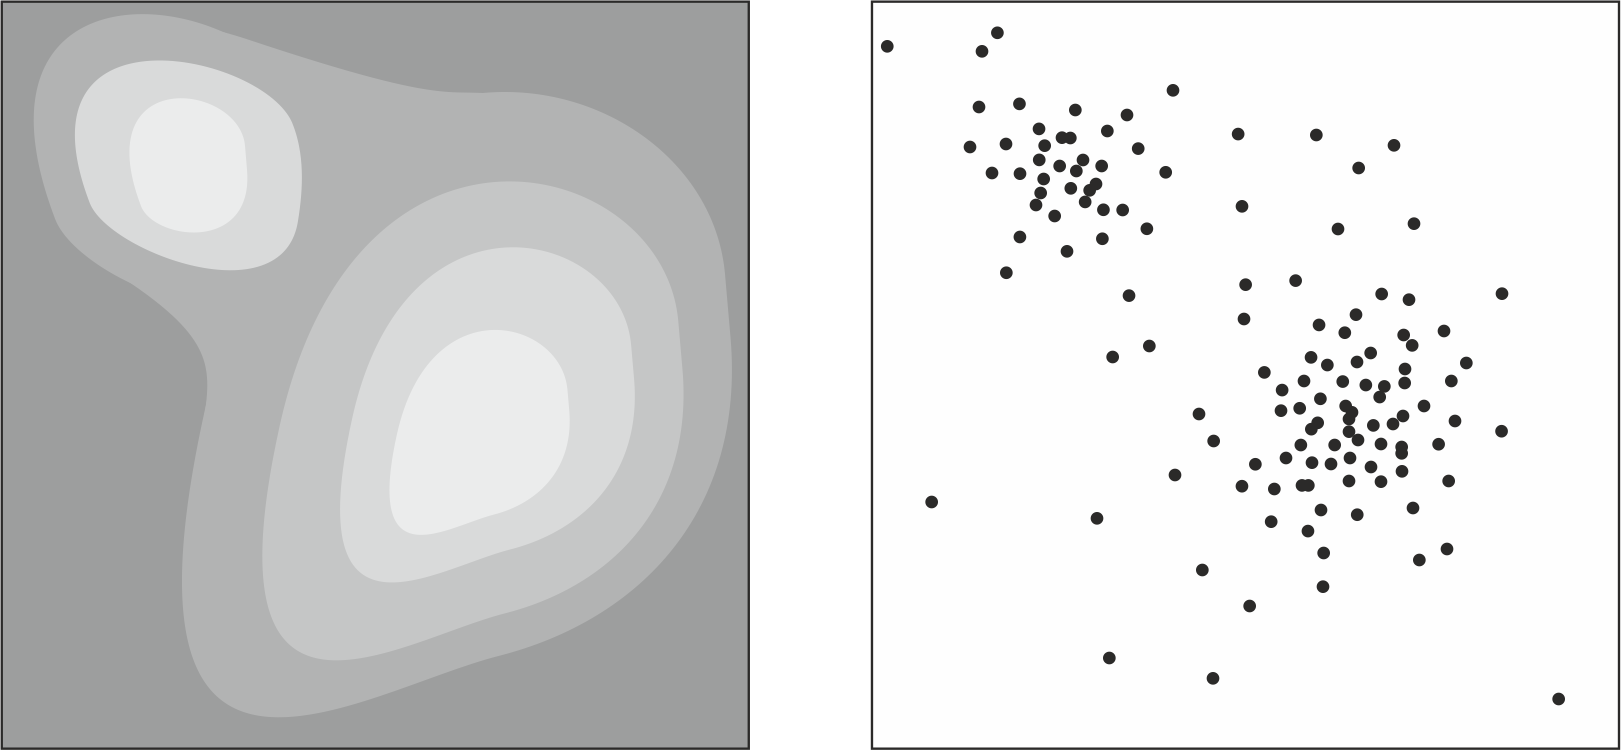
\includegraphics[width=\textwidth]{smath.png}
\caption{Illustration of sampling procedure. Left: The square represents the space ${\mathscr S}_{\rm math}$ and the shading is the probability distribution $\rho$ over it. The brighter the shading, the higher the probability. Right: We randomly distribute a set of $N$ points using $\rho$. In the limit $N \to \infty$ a uniform distribution $\tilde \rho$ on the points will reproduce the probabilities defined by $\rho$ on ${\mathscr S}_{\rm math}$ with a uniform measure. The set of points defines the new space ${\mathscr S}_{\rm phys}$. It has a non-trivial measure $\tilde \mu$ in ${\mathscr S}_{\rm math}$. Any correlations that were present in $\rho$ are thereby moved into the structure of ${\mathscr S}_{\rm phys}$. \protect{\label{fig}}}
\end{figure*}

Let us now take a subset $A$ of ${\mathscr S}_{\rm math}$ with non-zero volume (according to $\mu$), $A \subset {\mathscr S}_{\rm math}$. In the limit $N\to \infty$, we then have for the probability $P(A)$ of finding the system in that subset
\beqn
P(A) = \int_{A} d\lambda dX ~ \tilde \rho_{\rm Bell}(\lambda, X)   = \int_A d \lambda dX ~ \rho_{\rm Bell}(\lambda, X)~,
\eeqn
for any $A$.
This means that all probabilities calculated from $\rho$ on ${\mathscr S}_{\rm math}$ with uniform measure $\mu \equiv \mu_0$ are by construction identical to those of the uniform distribution $\tilde \rho$ with measure $\tilde \mu$. 

Finally, we define the new, physical state-space ${\mathscr S}_{\rm phys}:= \lim_{N\to \infty} {\mathscr S}_N$. Since $\tilde \mu \equiv 0$ on ${\mathscr S}_{\rm math} \setminus {\mathscr S}_{\rm phys}$, we discard the complement, only keep ${\mathscr S}_{\rm phys}$, and restrict the probability $\tilde \rho$ to ${\mathscr S}_{\rm phys}$.

Once we have done that, the entire information that was previously in $\rho$ has moved into the definition of the physical state-space ${\mathscr S}_{\rm phys}$. 
$\rho_{\rm Bell} = \rho \mu$ and $\tilde \rho_{\rm Bell} = \tilde \rho \tilde \mu$ give exactly the same probabilities. Since we never experimentally measure probability-densities but only probabilities, these two theories are physically indistinguishable. Both violate Statistical Independence as defined in Eq.\ (\ref{rhobell}). But $\tilde \rho(\lambda |X ) = \tilde \rho(\lambda)$, that is, the hidden variables are by construction uncorrelated on the new space. On ${\mathscr S}_{\rm phys}$, the theory would violate Eq.\ (\ref{rhobell}), but not Eq.\ (\ref{SI2}). 

It is in this sense that the common interpretation of Statistical Independence is wrong: On a state space with non-trivial measure, the hidden variables may not be correlated with the detector settings and yet the Statistical Independence assumption used for Bell's theorem will be violated. The common interpretation neglects the possibility that the theory is supermeasured rather than superdeterministic.

Moving the correlation into the definition of the physical state space is a simple way to avoid finetuning, the claim that the experimentally confirmed correlations are sensitive to small changes in the distribution (raised e.g. in \cite{Sen2020Superdet2,Wood2015FineTuning}). If the correlations are created by the intrinsic properties of the space itself, rather than the distribution over the space, then small changes just can't happen. This is the idea of Invariant Set Theory ({\sc IST}) \cite{Palmer2020Discretization} which we will discuss in more detail in Section \ref{IST}. Other reasons why the fine-tuning argument can fail were previously discussed in \cite{Hossenfelder2020SuperdeterminismGuide,Wharton2019Reformulations,Donadi2020SuperdetToy}.

\section{Statistical Independence in the CHSH inequality}
\label{CHSH}

Before turning to Invariant Set Theory as a natural example for a non-trivial measure, we will go through a simple example, the {\sc CHSH} inequality \cite{Clauser1969CHSH}.
The {\sc CHSH} setting describes a measurement of two entangled particles with two different detectors, commonly assigned to two observers, Alice ($A$) and Bob ($B$). The inequality states that any locally causal hidden variables theory which respects Statistical Independence fulfils
\begin{equation}
   \big| E(X_0,Y_0)-E(X_1,Y_0)+E(X_0,Y_1)+E(X_1,Y_1) \big| \leq 2~,
\end{equation}
where $X_{0/1}$ are detector settings on Alice's side and $Y_{0/1}$ are the detector settings on Bob's side. The quantum correlations $E(X_{0/1},Y_{0/1})$ are the expectation values of the results, $A(X_{0/1})$ and $B(Y_{0/1})$, where $A(X_{0/1})$ is Alice's result given Alice's setting $X_{0/1}$, and $B(Y_{0/1})$ is Bob's result given Bob's setting $Y_{0/1}$. 
We will consider the usual case in which there are only two possible measurement outcomes relative to those settings, $A(\cdot),B(\cdot) \in \{-1,+1 \}$.

In experimental tests of the {\sc CHSH} inequality, the correlations for four different combinations of settings are estimated from four separate sub-ensembles of particles. 
Statistical independence is then the assumption that 
\be
\label{SI3}
\tilde \rho (\lambda | X_0 Y_0) = \tilde \rho(\lambda | X_0 Y_1) = \tilde \rho(\lambda | X_1 Y_0) = \tilde \rho(\lambda | X_1 Y_1) = \tilde \rho(\lambda)~,
\ee
that is, the distribution of hidden variables does not depend on the (combination of) detector settings. We will assume that our hidden variables theory fulfils this assumption.

We will now explain how the {\sc CHSH} inequality can be violated in a hidden variables model by violating Statistical Independence but not statistical independence. For this, we first assume that the entangled state is represented by a hidden variable, $\lambda$, which has the probability distribution $\tilde \rho(\lambda,XY)$. And next, that the measurement outcome is determined by the hidden variable and the settings: $A(\lambda,X), B(\lambda,Y)$.

We will denote the space of all the hidden variables with $\Lambda$ and divide it up into subsets for each possible combination of detector settings and outcomes $\Lambda_{XY}^{AB}$. That is, the subset $\Lambda^{++}_{00}$ contains all $\lambda$s for setting $X_0Y_0$ that will give the result $A=+1,B=+1$, the subset $\Lambda^{+-}_{00}$ contains all $\lambda$s for setting $X_0Y_0$ that will give the result $A=+1,B=-1$, and so on.

However, we will next assume that the hidden variable cannot occur for two different combinations of measurement settings. If the variable $\lambda$ described the case with setting $X_0Y_0$, then the combination $(\lambda,X_0Y_1)$ is in ${\mathscr S}_{\rm math}$ but not in ${\mathscr S}_{\rm phys}$. This means that 
\beqn
\Lambda = \bigcup_{i,j,k,l} \Lambda^{ij}_{kl}\quad \mbox{for} \quad i,j \in \{+,-\}~\wedge~k,l \in \{0,1\}~,
\eeqn
but that these spaces are mutually disjoint
\beqn
\Lambda^{ij}_{kl} \cap \Lambda^{ab}_{cd} = \emptyset \quad \mbox{for} \quad ijkl \neq abcd~.
\eeqn

This does not contradict (\ref{SI3}) because statistical independence is a statement about the probability distribution. The probability distributions for the four different combinations of settings can be made similar to arbitrary precision, even though no value of $\lambda$ appears twice. 

Imagine for example that $\lambda$ is a real number from the interval $[0,1] \in {\mathbb{Q}}$. We randomly sample $N$ points from this interval using a uniform distribution and assign each to one of combinations of settings and outcomes, i.e. one of the $\Lambda^{ij}_{kl}$. The so-generated probability distributions will be statistically indistinguishable for $N\to \infty$ even though the probability that $\lambda$ appears for two different settings is zero. Note that this is the case regardless of how many of the $\lambda$'s we assign to each detector provided the cardinality of all subsets is the same. In the limit $N\to \infty$ the distribution for $\lambda$ conditioned on one of the detectors will just be uniform on each subspace $\Lambda^{ij}_{kl}$.

However, and here comes the important point, the measures of the subspaces $\Lambda^{ij}_{kl}$ don't have to be the same. All we need to do now is choose $\tilde \rho$ to be constant, and the measure of the space $\Lambda^{ij}_{kl}$ to be proportional to the quantum mechanical probability $P\Big(A(X_k)B(Y_l)|X_i Y_j\Big)$ (the constant of proportionality will cancel with the normalisation of $\tilde \rho$) for each possible combination of outcomes. Note that, since $\lambda$ together with the detector setting determines the outcome, the outcome isn't an independent variable. As a result, if we want to calculate the expectation value for a certain combination of measurement settings in the hidden variables model, we have
\beqn
E(X_k,Y_l) &=& 
\sum_{AB} \int_{\Lambda^{AB}_{kl}} \hspace*{-0.3cm} d \lambda~ A(\lambda,X_k) B(\lambda,Y_l) \tilde \rho(\lambda) \tilde \mu(\lambda | X_kY_l) \nonumber \\
&=& \sum_{AB} A(X_k) B(Y_l) P\Big(A(X_k)B(Y_l)|X_k Y_l\Big) ~,
\eeqn
which reproduces the correlations of quantum mechanics.

Again it might seem rather trivial: We have just pushed the quantum mechanical correlation into the definition of the physical state space and then uniformly sampled the hidden variables over this space. This way, statistical independence is respected because the correlation comes from the definition of the space rather than from the distribution over it. 


The above example can be generalised straight-forwardly to any quantum mechanical measurement, regardless of what variables are measured in what order or how many detectors there are. The above construction will always give the exact same result as quantum mechanics. In particular it will obey the same bounds and violate all other inequalities just the same as quantum mechanics. 

Of course this example is somewhat pointless because we didn't specify the model sufficiently to even know whether it's locally causal. However, any deterministic hidden variables theory that violates local causality can be made locally causal on the expense of violating Statistical Independence. We have now further shown that -- contrary to what is often stated -- violating Statistical Independence does not necessarily require correlations between the hidden variables and measurement settings.

This isn't the only way to reproduce quantum mechanics with a locally causal and deterministic model without fine-tuning \cite{Donadi2020SuperdetToy} but it is a nice example to see just why the distribution of the hidden variables is not fine-tuned. It is uniform on the sample-space, and the sample-space just describes what happens in reality. If the detector setting is one thing, it is not also another thing. The correlations come from the sample-space itself. And the information that goes into the construction of the sample-space is just the same as in quantum mechanics. Hence, this model is exactly as fine-tuned or not fine-tuned as quantum mechanics. That is to say, a rational reader who has no quarrels with quantum mechanics should have no quarrels with this model either.


\section{Invariant Set Theory}
\label{IST}


\subsection{The Mathematical Basis of Invariant Set Theory}
\label{istmath}

Invariant Set Theory ({\sc IST}) \cite{Palmer2020Discretization,Palmer1995Spin,Palmer2009ISP} is a putative theory of quantum physics based on the assumption that the universe is a causal deterministic dynamical system whose state-space is a fractal set, $I_U$. This fractal set corresponds to ${\mathscr S}_{\rm phys}$ of the previous section. It is invariant under the action of dynamical equations: if a point lies on $I_U$, its time evolution always lies on $I_U$; if a point does not lie on $I_U$ its time evolution never will and never has. The nontrivial measure $\tilde \mu$ is the measure of this invariant set. It is sometimes called the invariant measure. Each trajectory of $I_U$ actually comprises a Cantor Set's worth of trajectories. As such $\tilde \mu$ is a Hausdorff measure \cite{Rogers1998Hausdorff} -- a generalisation of Lebesgue measure for spaces with non-integer dimension. 

Notably, if the state space is a fractal, it has gaps. (Indeed one could say it is mostly gaps since the set has measure zero in the continuum embedding space.) In {\sc IST}, the states in the gaps are not ontic, they are counterfactual states that are mathematically possible (and hence lie in ${\mathscr S}_{\rm math}$), but are inconsistent with the assumed laws of physics (and hence do not lie in ${\mathscr S}_{\rm phys}$). With respect to a Euclidean metric on ${\mathscr S}_{\rm math}$, the non-ontic states are arbitrarily close to the ontic states. That is, perturbations (which are tiny with respect to the Euclidean metric) will generically take an ontic state to one that is inconsistent with the assumed laws of physics. This does not make the theory fine-tuned as perturbations which take ontic states off the invariant set are necessarily $p$-large with respect to a $p$-adic norm. Such a norm, and associated metric, is the natural one to use on a fractal geometry. And if {\rm IST} is not fine tuned, it cannot be conspiratorial. 

The fractal structure that underpins $I_U$ is further assumed to be isomorphic to the $p$-adic integers, for some very large $p$. The theory of dynamical systems defined on $p$-adic numbers is an established part of arithmetic dynamics (see e.g. \cite{Woodcock1998padic} and references therein). 

As a consequence of this fractal structure, an ensemble-based probabilistic state of the system in {\sc IST} can be expanded in the basis of detector eigenstates $|A_j \rangle$ in the form:
\be
|\psi\rangle = a_1 |A_1\rangle + a_2|A_2\rangle \ldots + a_J |A_J\rangle~,
\ee
where the coefficients as usual square to 1, ie $\sum_j a_j a^*_j =1$ and the star denotes complex conjugation.
The crucial difference to standard quantum theory is that in {\sc IST} the complex amplitudes $a_j$ belong to a subset of the complex numbers $a_j \in \mathbb C_p, \mathbb C_p \subset \mathbb C$. The elements of $\mathbb C_p$ obey rationality restrictions on the coefficients (and so do not form a field). Specifically, if we write $a_j$ in polar form $a_j=R_j e^{i \phi_j}$ then the fractal structure of $I_U$ demands
\beqn
\label{finite}
R^2_j=m_j/p; \ \ \ 
\phi_j = 2\pi n_j/p~,
\eeqn
where $m_j,n_j,p \in {\mathbb N}_0$, $m_j,n_j < p$.

In the limit $p \rightarrow \infty$, the set of such ``rational'' Hilbert states is dense in the projection of the quantum mechanical Hilbert-space. From this point of view, for large enough $p$, {\sc IST} can be made as experimentally indistinguishable from quantum theory as one likes. This makes it difficult to devise experimental tests for this idea. Such tests must ultimately be based on the fact that, at the end of the day, $p$ is some finite number \cite{Hance2021ExpIST}. 

However, no matter how large is $p$, the state-space of this theory will continue to have gaps. That is to say, the limit $p \rightarrow \infty$ is singular: quantum mechanics does not correspond to {\sc IST} in the large $p$ limit. Importantly, no matter how large is $p$, ensembles of trajectories described by Hilbert States where the complex amplitudes do not belong to $\mathbb C_p$, do not lie on $I_U$. As such, these trajectories have the measure $\tilde \mu=0$ in the continuous embedding space. 

With this {\sc IST} explains why it is impossible to simultaneously measure conjugated variables in quantum mechanics with certainty. In quantum theory, this is a consequence of having non-commuting operators acting on a Hilbert-space, but is otherwise unexplained. In {\sc IST} this arises in a deterministic framework because of the geometric structure of the invariant set and associated fractal measure. The incomplete algebraic structure of ${\mathbb C}_p$ reflects the ``gappy'' geometric structure of $I_U$. For example, superpositions of two states which are in ${\mathbb C}_p$ are generically not also in ${\mathbb C}_p$. 

\subsection{The CHSH Inequality in Invariant Set Theory}
\label{CHSHIST}

We will now explain how {\sc IST} violates the {\sc CHSH} inequality.

In {\sc IST}, if we keep the setting of the first detector fixed (say, at $X_0$), then the settings $Y_0$ and $Y_1$ of the second detector cannot both be on the set if $Y_0 \neq Y_1$. If $Y_0$ was on the set together with $X_0$, then $Y_1$ won't be on it, or the other way round. One of them is not physically possible. This property is a consequence of the rationality requirement on the amplitudes and phases and a number-theoretic result known as Niven's theorem
 \cite{Niven1956irrational,Jahnel2010Sines}:
\begin{quote}
{\bf Niven's Theorem:}
 \emph{Let $\phi/2\pi \in \mathbb{Q}$. Then $\cos \phi \notin \mathbb{Q}$ except when $\cos \phi =0, \pm \frac{1}{2}, \pm 1$.}
\end{quote}
If the first combination of settings, ($X_0Y_0$) for given $\lambda$, fulfils the rationality condition, then the second one, $(X_0Y_1)$ for the same $\lambda$, can't fulfil it; it is associated with a state in ${\mathscr S}_{\rm math}$ where $\tilde \mu=0$. 

This means that 
\beqn
\tilde \rho_{\rm Bell} (\lambda | X_0 Y_0) \ne 0 \implies \tilde \rho_{\rm Bell}(\lambda | X_0 Y_1) = \tilde \rho_{\rm Bell}(\lambda | X_1 Y_0)=0 \\
\tilde \rho_{\rm Bell} (\lambda | X_1 Y_0) \ne 0 \implies \tilde \rho_{\rm Bell}(\lambda | X_0 Y_0) = \tilde \rho_{\rm Bell}(\lambda | X_1 Y_1)=0
\eeqn
etc. However, this does not imply
\beqn
\tilde \rho(\lambda | X_0 Y_0) \ne 0 \implies \tilde \rho(\lambda | X_0 Y_1) = \tilde \rho(\lambda | X_1 Y_0)=0\\
\tilde \rho(\lambda | X_1 Y_0) \ne 0 \implies \tilde \rho(\lambda | X_0 Y_0) = \tilde \rho(\lambda | X_1 Y_1)=0
\eeqn
etc.

Now because the statistics of trajectories in {\sc IST} can be represented by complex Hilbert vectors over $\mathbb C_p$ for large $p$, the measures of the spaces $\Lambda^{ij}_{kl}$ introduced in Section \ref{CHSH} are proportional to the quantum mechanical probabilities $P\big(A(X_k)B(Y_l)|X_k Y_l\big)$. Hence {\sc IST} reproduces the correlations of quantum mechanics.

\subsection{Free Will}
\label{free}


As mentioned at the beginning, Statistical Independence is sometimes called the Free Will and/or Free Choice assumption. This refers to the notion that if, for example, Alice actually chose $X_0$ and Bob $Y_0$, then, keeping $\lambda$ and Alice’s choice fixed, Bob could have chosen $Y_1$ instead -- he had the freedom to have done otherwise. But as we have also discussed, such a counterfactual state is incompatible with {\sc IST}: If Bob actually chose $Y_0$, then the state corresponding to the triple $(\lambda, X_0, Y_1)$ is not in the physical state-space; it corresponds to a point in ${\mathscr S}_{\rm math}$ where $\tilde \mu=0$. 

But does this constraint actually have anything to do with free choice? In a deterministic framework, like {\sc IST}, free will can at best be interpreted as the absence of constraints that could prevent an agent from doing as they please. But there is nothing in {\sc IST} that would prevent an agent from doing as he or she pleases any more than this is always the case in any deterministic theory -- the laws of nature always constrain what we can do. And just as it is possible to violate Statistical Independence without violating statistical independence, it is possible to violate Free Choice without violating free choice -- remember that after all Free Choice is just a fancy name for Statistical Independence. That is, in {\sc IST} Bob can freely chose \emph{among the physically possible options} in the sense that there is no constraint on them. 

However, some may not accept this argument. For them, the notion that “I could have done otherwise” is a very visceral and deeply held belief. Such people would not even countenance the possibility that Free Choice is somehow violated -- it is strictly off limits (and rejected in one line in many quantum foundations discussions). Why is this? A possible answer has been proposed in \cite{Palmer2020Brain}. If quantum processes play an essential role in human cognition, for which there is evidence, and if IST is a viable theory for such processes, then we humans may have some mental cognition of neighbouring trajectory segments on $I_U$. In some of these neighbouring trajectories we indeed did otherwise, and our cognition therefore concludes that we might have done otherwise. On the other hand, it is plausible that this cognition is not so finely developed that we are able to mentally distinguish neighbouring trajectories which lie on the invariant set from those that lie off the invariant set. (In the example above, the triple $(\lambda, X_1, Y_1)$ corresponds to a counterfactual world lying on $I_U$ even though the worlds corresponding to $(\lambda, X_0, Y_1)$ and $(\lambda, X_1, Y_0)$ do not.) That is to say, our cognitive ability to discriminate between counterfactual worlds on $I_U$ and counterfactual worlds off $I_U$ may be poor. It is this somewhat indiscriminate cognitive sense of the existence of such counterfactual worlds that may give many of us the generic belief that we could have done otherwise. 

\section{Conclusion}

While Bell's theorem is often said to imply that local causality (which is violated by standard quantum mechanics) cannot be restored with a deterministic hidden variables theory, this is only correct if the hidden-variables theory respects Statistical Independence. Violations of Statistical Independence are commonly interpreted as implying a correlation between the measurement settings and the hidden variables which determine the measurement outcomes. However, as we have shown here, one can violate the Statistical Independence assumption in Bell's theorem without any correlations between the measurement outcomes and the hidden variables. The violations of Statistical Independence can instead come about by the geometry of the underlying state space. We have argued that this is a simple way to see that violating Statistical Independence does not require fine tuning.

\bigskip

\textit{Acknowledgements---}
We thank Sophie Inman and John Rarity for useful discussions. TP is funded by a Royal Society Research Professorship. SH acknowledges support by the Deutsche Forschungsgemeinschaft (DFG, German Research Foundation) under grant number HO 2601/8-1. JRH is supported by the University of York's EPSRC DTP grant EP/R513386/1, and the EPSRC Quantum Communications Hub (funded by the EPSRC grant EP/M013472/1).

\bibliographystyle{unsrt}
\bibliography{ref.bib}

\end{document}